\documentclass[12pt,a4paper]{article}
\usepackage[utf8]{inputenc}
\usepackage[spanish,es-tabla]{babel}
\usepackage{geometry}
\usepackage{graphicx}
\usepackage{multirow}
\usepackage{tabularx}
\usepackage{mathptmx}
\usepackage{fancyhdr}
\usepackage{array}
\usepackage[table]{xcolor}
\usepackage{titlesec}
\usepackage{setspace}
\usepackage{microtype}
\usepackage{lastpage}
\usepackage{booktabs}
\usepackage{enumitem}
\usepackage{amsmath}
\usepackage{amsfonts}
\usepackage{amssymb}

\usepackage{float}
\usepackage{placeins}
\usepackage{tikz}
\usepackage{pgfplots}
\pgfplotsset{compat=1.17}
\usetikzlibrary{arrows.meta,positioning,shapes.geometric,calc}

\graphicspath{{images/}{../images/}{./}}

\geometry{
    top=4.7cm,
    bottom=2.5cm,
    left=2.5cm,
    right=2.5cm,
    headheight=3.9cm,
    headsep=0.4cm
}

\setstretch{1.15}
\setlength{\parindent}{0pt}
\setlength{\parskip}{0.45em}
\setlength{\tabcolsep}{4pt}

\titleformat{\section}
  {\normalfont\fontsize{12}{14.5}\bfseries}{\thesection.}{0.6em}{\uppercase}
\titlespacing*{\section}
  {0pt}{1.8ex plus 0.4ex minus 0.2ex}{0.6ex plus 0.2ex}

\titleformat{\subsection}
  {\normalfont\fontsize{11.5}{13.5}\bfseries}{\thesubsection.}{0.5em}{}
\titlespacing*{\subsection}
  {0pt}{1.4ex plus 0.3ex minus 0.1ex}{0.4ex plus 0.1ex}

\titleformat{\subsubsection}
  {\normalfont\fontsize{10.5}{12.5}\bfseries\itshape}{\thesubsubsection.}{0.4em}{}
\titlespacing*{\subsubsection}
  {0pt}{1.1ex plus 0.2ex minus 0.1ex}{0.3ex plus 0.1ex}

\newcolumntype{Y}{>{\centering\arraybackslash}X}
\newcolumntype{L}{>{\raggedright\arraybackslash}X}
\newcolumntype{C}{>{\centering\arraybackslash}X}

\definecolor{headerblue}{RGB}{26, 54, 93}
\definecolor{darkblue}{RGB}{43, 108, 176}
\definecolor{lightgraybg}{RGB}{248, 248, 248}
\definecolor{tableheader}{RGB}{232, 238, 246}
\definecolor{navyheader}{RGB}{0, 32, 96}
\definecolor{lineblue}{RGB}{0, 102, 204}
\definecolor{areablue}{RGB}{220, 236, 252}
\definecolor{lcsred}{RGB}{217, 56, 41}
\definecolor{lcigreen}{RGB}{46, 125, 50}
\definecolor{lciorange}{RGB}{230, 81, 0}
\definecolor{ishikawared}{RGB}{160, 0, 0}

\tikzset{
    catbox/.style={draw, fill=tableheader, font=\footnotesize\bfseries, minimum width=2.8cm, minimum height=0.65cm, align=center},
    efectobox/.style={draw=ishikawared!90!black, line width=1.2pt, fill=ishikawared, text=white, font=\small\bfseries, align=center, inner sep=6pt, text width=3.8cm},
    causetext/.style={font=\scriptsize, align=right, text=black!90}
}

\newcommand{\docCodigo}{TI-SIGE-ENT-F3-009}
\newcommand{\docVersion}{1.0}
\newcommand{\docProceso}{IMPLEMENTACIÓN DE SOFTWARE / MATRIZ DINÁMICA DE ACTIVIDADES}
\newcommand{\docElaboracion}{28/09/2026}
\newcommand{\docRevision}{28/09/2026}
\newcommand{\docTitulo}{DESARROLLO DE LA MATRIZ DINÁMICA}
\newcommand{\docOrganizacion}{FACULTAD DE INGENIERÍA EN SISTEMAS, ELECTRÓNICA E INDUSTRIAL}
\newcommand{\docSubOrganizacion}{CARRERA DE INGENIERÍA DE SOFTWARE}

\newcommand{\encabezadofrecuente}{%
    \renewcommand{\arraystretch}{1.15}%
    \noindent\makebox[\textwidth][c]{%
    \begin{tabularx}{\textwidth}{|>{\centering\arraybackslash}m{2.8cm}|Y|>{\centering\arraybackslash}m{4.8cm}|}
        \hline
        \multirow{4}{2.8cm}{\centering\raisebox{-1.15cm}{
\includegraphics[width=2.5cm,height=2.0cm,keepaspectratio]{images/logo.png}}}
        & \textbf{\fontsize{9}{11}\selectfont \docOrganizacion} 
        & \textbf{\fontsize{8}{10}\selectfont CÓDIGO:} \fontsize{8}{10}\selectfont \docCodigo \\
        \cline{3-3}
        & \textbf{\fontsize{8.5}{10.5}\selectfont \docSubOrganizacion} 
        & \textbf{\fontsize{8}{10}\selectfont VERSIÓN:} \fontsize{8}{10}\selectfont \docVersion \\
        \cline{2-3}
        & \textbf{\fontsize{8}{10}\selectfont PROCESO:} \fontsize{8}{10}\selectfont \docProceso 
        & \textbf{\fontsize{8}{10}\selectfont ELABORACIÓN:} \fontsize{8}{10}\selectfont \docElaboracion \\
        \cline{2-3}
        & \textbf{\fontsize{8.5}{10.5}\selectfont \docTitulo} 
        & \textbf{\fontsize{8}{10}\selectfont ÚLTIMA REVISIÓN:} \fontsize{8}{10}\selectfont \docRevision \\
        \hline
    \end{tabularx}%
    }%
}

\pagestyle{fancy}
\fancyhf{}
\fancyhead[C]{\encabezadofrecuente}
\fancyfoot[C]{\fontsize{10}{12}\selectfont Página \thepage\ de \pageref{LastPage}}
\renewcommand{\headrulewidth}{0pt}

\begin{document}

\noindent{\fontsize{10.5}{12.5}\selectfont \textbf{Integrantes:} Heidi Villavicencio \quad$\vert$\quad Steeven Toala \quad$\vert$\quad Nixon Hurtado \quad$\vert$\quad Andrea Vásquez}

\vspace{0.25cm}

\section{Título}
\textbf{Denominación Oficial del Entregable:} Desarrollo de la Matriz Dinámica de Actividades -- Código EDT: 3.9

\section{Introducción}
La Tabla 1 del formato institucional del Sistema de Gestión de la Calidad (\texttt{UTA-SGC-A-2-1-P7-T1}), correspondiente a la Planificación de Actividades y su Control Semestral, constituye el núcleo aritmético y normativo de la rendición docente en la FISEI. En los formatos manuales anteriores en Microsoft Word, esta sección presentaba graves fallas operativas: sumas asimétricas que no totalizaban el 100\%, cálculo erróneo del avance acumulado e inconsistencias en la distribución semanal. Para resolver definitivamente esta problemática, se desarrolló el componente interactivo reactivo \texttt{MatrizActividadesTable.jsx}, el cual permite crear, editar y eliminar actividades académicas con recálculo matemático instantáneo de ponderaciones, selector matricial de 16 semanas y validación de suma exacta al 100\%.

\section{Objetivo}
\subsection{Objetivo General}
Desarrollar, integrar y validar el componente interactivo de Matriz Dinámica de Actividades con cálculo automático en tiempo real de ponderación ($\sum P_i = 100\%$) y cronograma semanal para el sistema SIGE.
\subsection{Objetivos Específicos}
\begin{itemize}[leftmargin=1.5em, itemsep=2pt]
    \item Construir la tabla interactiva reactiva utilizando el hook \texttt{useReducer} para gestión inmutable de filas.
    \item Implementar el validador aritmético en tiempo real de ponderación porcentual y horas semanales.
    \item Integrar el selector de cronograma semestral de 16 semanas con cálculo de avance ponderado.
\end{itemize}

\section{Alcance}
\subsection{Límites del Entregable (In-Scope)}
\begin{itemize}[leftmargin=1.5em, itemsep=2pt]
    \item Componente \texttt{MatrizActividadesTable.jsx} plenamente operativo en el Paso 3 del Wizard.
    \item Botones interactivos ``+ Agregar Actividad'', ``+ Sugerir con IA'', eliminación de fila y cálculo de avance.
    \item Clasificación estricta por áreas del SGC: Docencia, Investigación, Vinculación y Gestión.
\end{itemize}
\subsection{Exclusiones (Out-of-Scope)}
\begin{itemize}[leftmargin=1.5em, itemsep=2pt]
    \item Almacenamiento físico de archivos binarios de verificación (desarrollado en EDT 3.11).
\end{itemize}

\section{Definiciones}
\begin{itemize}[leftmargin=1.5em, itemsep=2pt]
    \item \textbf{Matriz Dinámica SGC:} Componente de interfaz de tipo hoja de cálculo ligera reactiva que ejecuta operaciones aritméticas de agregación sin recargar la página.
    \item \textbf{Ponderación de Actividad ($P_i$):} Peso porcentual asignado a una labor específica dentro del periodo semestral, cuya sumatoria global debe ser exactamente $100.00\%$.
    \item \textbf{Medio de Verificación:} Evidencia documental auditable (e.g., sílabos, actas, certificados) que justifica la ejecución y cumplimiento de una actividad.
    \item \textbf{Cronograma Semestral Matricial:} Matriz booleana de 16 columnas que representa la planificación temporal semana a semana de cada actividad docente.
\end{itemize}

\section{Responsabilidades}
\begin{itemize}[leftmargin=1.5em, itemsep=2pt]
    \item \textbf{Andrea Vásquez (Responsable EDT 3.9):} Desarrollo del componente interactivo de la matriz y algoritmos de cálculo.
    \item \textbf{Steeven Toala (Líder Técnico):} Verificación de fórmulas matemáticas de ponderación y persistencia inmutable.
    \item \textbf{Heidi Villavicencio (UI/UX):} Optimización visual, accesibilidad de la tabla y diseño de badges de estado.
    \item \textbf{Ing. Paulo Torres (Docente Evaluador):} Aprobación de la fidelidad con la Tabla 1 del formato oficial SGC.
\end{itemize}

\section{Normativa Legal y Técnica}
\subsection{Marco Legal Ecuatoriano}
\begin{itemize}[leftmargin=1.5em, itemsep=2pt]
    \item \textbf{Ley Orgánica de Educación Superior (LOES), Art. 122 y 149:} Obligatoriedad de registrar fielmente las actividades docentes planificadas y ejecutadas.
    \item \textbf{Reglamento de Régimen Académico (RRA - CES), Art. 45:} Distribución de la jornada de trabajo del personal académico en docencia, vinculación e investigación.
    \item \textbf{Formato Oficial UTA-SGC-A-2-1-P7-T1 y T2:} Estructura obligatoria de la Matriz de Actividades y Medios de Verificación.
\end{itemize}
\subsection{Normas Técnicas Internacionales}
\begin{itemize}[leftmargin=1.5em, itemsep=2pt]
    \item \textbf{ISO 9001:2015, Cláusula 7.5:} Aseguramiento de la integridad de datos cuantitativos en registros de calidad.
    \item \textbf{ISO/IEC 25010:2011:} Exactitud en cálculos numéricos y prevención de errores humanos de entrada.
\end{itemize}

\section{Método, Políticas y Contenidos}
\subsection{Enfoque Metodológico}
Para garantizar inmutabilidad, predictibilidad y rendimiento óptimo en la manipulación de filas complejas, se empleó el hook \texttt{useReducer} de React con acciones tipadas (\texttt{ADD\_ROW}, \texttt{UPDATE\_FIELD}, \texttt{TOGGLE\_WEEK}, \texttt{REMOVE\_ROW}, \texttt{CALCULATE\_TOTALS}). Las fórmulas aritméticas operan en tiempo real con precisión de dos decimales:
\begin{equation}
    P_{\text{total}} = \sum_{i=1}^{n} P_i, \qquad A_G = \sum_{i=1}^{n} \left( \frac{P_i}{100} \times A_i \right)
\end{equation}
donde $P_{\text{total}}$ es la sumatoria de ponderaciones (obligatoriamente $100.00\%$), $A_i$ es el porcentaje de avance reportado para la actividad $i$, y $A_G$ es el avance global acumulado del informe.

\subsection{Políticas de Calidad de la Matriz Dinámica}
\begin{enumerate}[leftmargin=1.5em, itemsep=2pt]
    \item \textbf{Política del 100\% Estricto:} Si la suma de ponderaciones difiere de $100.00\%$ (e.g., $95\%$ o $105\%$), el sistema bloquea el paso de guardado final y resalta la diferencia en color rojo carmesí.
    \item \textbf{Política de Medio de Verificación Obligatorio:} Cada actividad registrada debe declarar al menos un medio de verificación auditable y específico.
    \item \textbf{Política de Coherencia Cronológica:} Toda actividad debe tener marcada al menos una de las 16 semanas del semestre lectivo.
    \item \textbf{Política de Inmutabilidad de Filas:} Las operaciones sobre la tabla no mutan el estado directamente, previniendo condiciones de carrera (\textit{race conditions}) en el navegador.
\end{enumerate}

\begin{figure}[H]
    \centering
    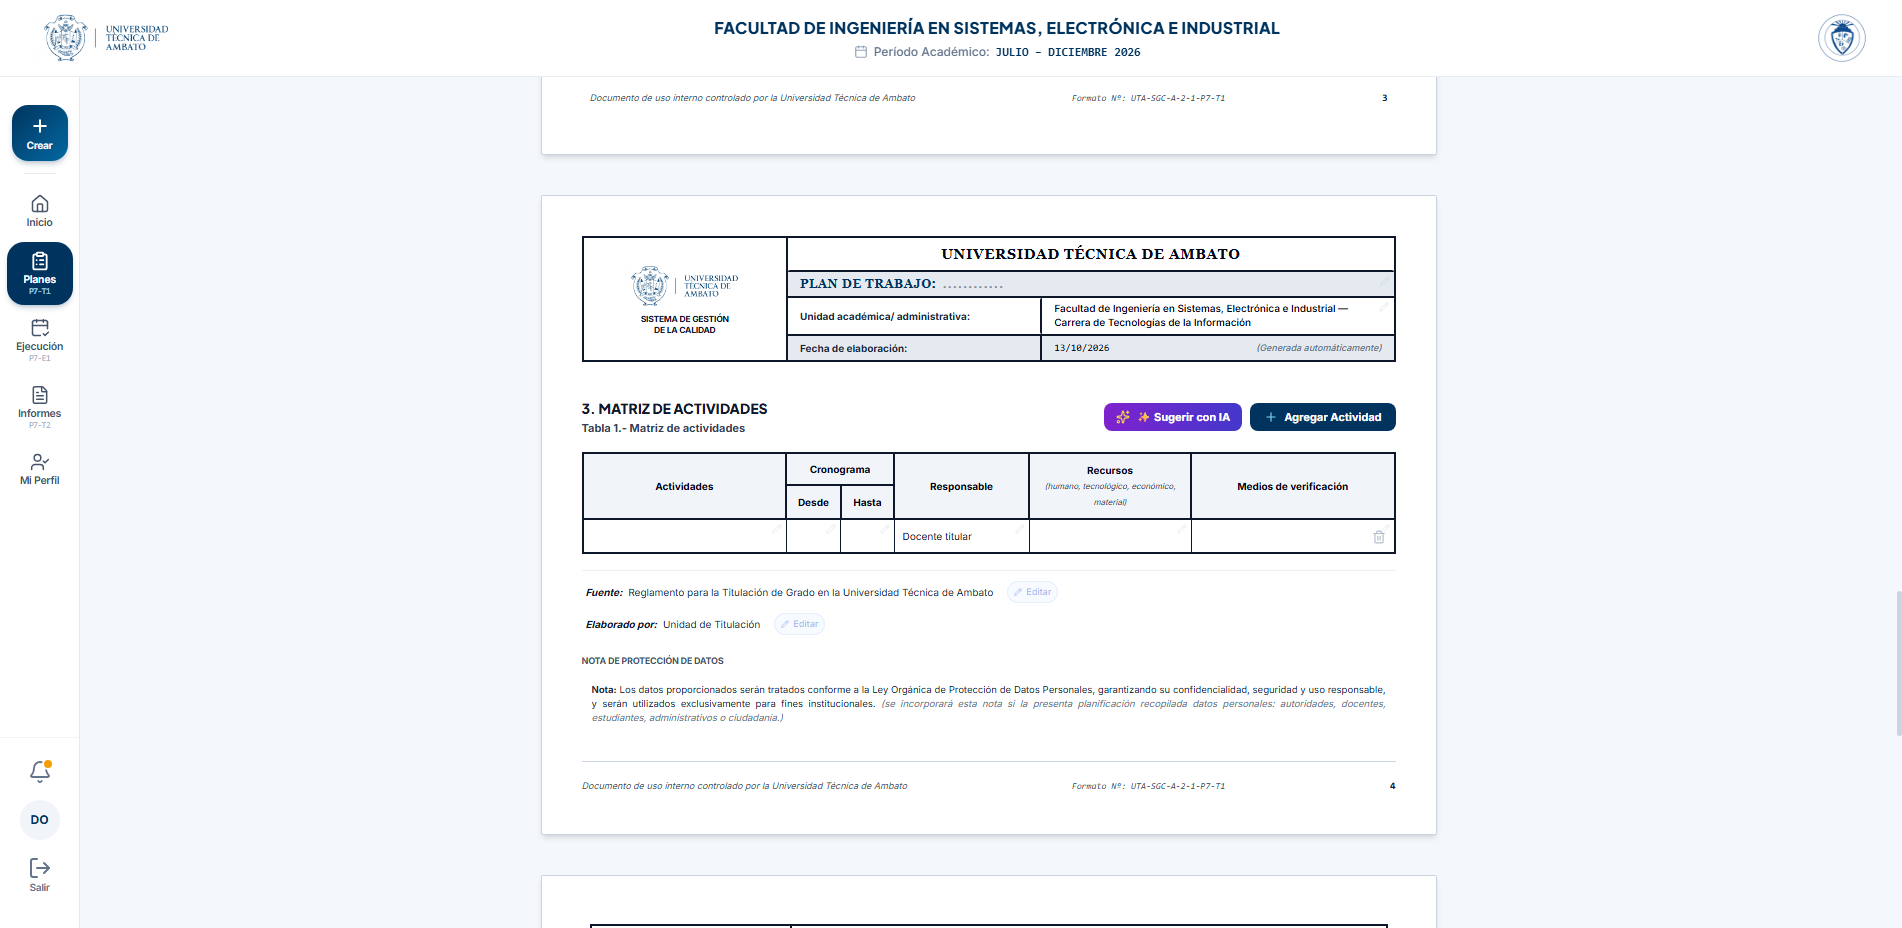
\includegraphics[width=0.88\textwidth,height=6.2cm,keepaspectratio]{images/sige_matriz_dinamica_actividades.png}
    \caption{Captura Real del Componente Interactivo de la Matriz Dinámica de Actividades SGC en SIGE.}
    \label{fig:matriz_dinamica_real}
\end{figure}
\FloatBarrier

\section{Descripción de actividades}
\subsection{Matriz Oficial de Datos de Actividades del Plan Docente (Tabla 1 SGC)}
A continuación se presenta la tabla formal con el conjunto completo de actividades académicas modeladas en el sistema, totalizando exactamente el 100\% de ponderación y cubriendo la carga horaria semanal:

\begin{table}[H]
\centering
\small
\renewcommand{\arraystretch}{1.15}
\begin{tabularx}{\textwidth}{|c|>{\raggedright\arraybackslash\bfseries}m{2.8cm}|X|c|c|m{2.8cm}|}
\hline
\rowcolor{tableheader}
\textbf{N°} & \textbf{Área SGC} & \textbf{Actividad Específica Planificada} & \textbf{Horas} & \textbf{Pond.} & \textbf{Medio de Verificación} \\
\hline
1 & Docencia & Dictado de Cátedra: Ingeniería de Software I y II & 16 h & 40.00\% & Registro de Asistencia, Sílabo. \\
\hline
2 & Docencia & Preparación de clases, material didáctico y evaluaciones & 8 h & 20.00\% & Guías de Taller, Rúbricas. \\
\hline
3 & Docencia & Tutorías Académicas y atención a estudiantes & 4 h & 10.00\% & Bitácora de Tutorías, Actas. \\
\hline
4 & Investigación & Proyecto I+D: Desarrollo de Plataforma de Calidad SIGE & 6 h & 15.00\% & Avance de Proyecto, Código Git. \\
\hline
5 & Gestión & Comisión Académica y Acreditación de Carrera & 4 h & 10.00\% & Actas de Reunión de Comisión. \\
\hline
6 & Vinculación & Capacitación comunitaria en alfabetización digital & 2 h & 5.00\% & Certificados, Nómina asistentes. \\
\hline
\multicolumn{3}{|r|}{\textbf{TOTALES CONSOLIDADOS:}} & \textbf{40 h} & \textbf{100.00\%} & \textbf{Validación SGC: APROBADA} \\
\hline
\end{tabularx}
\caption{Matriz oficial de actividades académicas del plan semestral P7-T1.}
\label{tab:matriz_actividades_datos}
\end{table}

\subsection{Matriz de Distribución del Cronograma Semanal (Semanas 1 a 16)}
\begin{table}[H]
\centering
\footnotesize
\renewcommand{\arraystretch}{1.15}
\begin{tabularx}{\textwidth}{|c|X|c|c|c|c|}
\hline
\rowcolor{tableheader}
\textbf{N°} & \textbf{Actividad Planificada} & \textbf{Sem. 1--4} & \textbf{Sem. 5--8} & \textbf{Sem. 9--12} & \textbf{Sem. 13--16} \\
\hline
1 & Dictado de Cátedra (Cursos Teóricos y Prácticos) & Activo & Activo & Activo & Activo \\
\hline
2 & Preparación de clases y diseño de instrumentos & Activo & Activo & Activo & Activo \\
\hline
3 & Tutorías Académicas individuales y grupales & Activo & Activo & Activo & Activo \\
\hline
4 & Desarrollo del Proyecto de Investigación SIGE & Activo & Activo & Activo & Activo \\
\hline
5 & Sesiones de Comisión Académica y Aseguramiento & Quincenal & Quincenal & Quincenal & Quincenal \\
\hline
6 & Talleres de Vinculación con la Sociedad & Inactivo & Activo & Activo & Cierre \\
\hline
\end{tabularx}
\caption{Cronograma de ejecución semestral distribuido en 16 semanas.}
\end{table}

\section{Firmas de Responsabilidad}

\noindent
\renewcommand{\arraystretch}{1.2}
\begin{tabularx}{\textwidth}{|>{\raggedright\arraybackslash}m{2.9cm}|>{\raggedright\arraybackslash}X|>{\centering\arraybackslash}m{4.6cm}|>{\centering\arraybackslash}m{2.3cm}|}
    \hline
    \rowcolor{tableheader}
    \textbf{ACCIÓN} & \textbf{NOMBRE Y CARGO} & \textbf{FIRMA} & \textbf{FECHA} \\
    \hline
    \textbf{Elaborado por:} & Heidi Villavicencio\newline Analista de Calidad / UI-UX & \parbox[c]{4.4cm}{\centering\vspace{4pt}
\includegraphics[height=1.5cm,width=4.0cm,keepaspectratio]{images/firma_heidi.png}\vspace{4pt}} & 28/09/2026 \\
    \hline
    \textbf{Revisado por:} & Steeven Toala\newline Líder de Proyecto / Arquitecto & \parbox[c]{4.4cm}{\centering\vspace{4pt}
\includegraphics[height=1.5cm,width=4.0cm,keepaspectratio]{images/firma_steveen.png}\vspace{4pt}} & 28/09/2026 \\
    \hline
    \textbf{Aprobado por:} & Ing. Paulo Torres, Mg.\newline Docente Evaluador -- Gestión Proyectos & \parbox[c]{4.4cm}{\centering\vspace{8pt}\textbf{\textcolor{gray!80}{\scriptsize [ PENDIENTE DE APROBACIÓN ]}}\vspace{8pt}} & \textbf{\textcolor{gray!90}{Pendiente}} \\
    \hline
\end{tabularx}

\vspace{0.4cm}

\section{Control de Cambios}

\noindent
\renewcommand{\arraystretch}{1.2}
\begin{tabularx}{\textwidth}{|>{\hsize=0.45\hsize\centering\arraybackslash}X|>{\hsize=1.55\hsize\raggedright\arraybackslash}X|>{\hsize=1.2\hsize\raggedright\arraybackslash}X|>{\hsize=0.8\hsize\centering\arraybackslash}X|}
    \hline
    \rowcolor{tableheader}
    \textbf{Versión} & \textbf{Descripción del cambio} & \textbf{Responsable del cambio} & \textbf{Fecha de aprobación} \\
    \hline
    1.0 & Emisión inicial del entregable según EDT del Tablero Trello & Equipo de Proyecto SIGE & 28/09/2026 \\
    \hline
\end{tabularx}

\vspace{0.4cm}

\section{Anexos}

\subsection*{Anexo 1: Ficha Técnica de la Tarea EDT 3.9 en el Tablero Trello}
\begin{table}[H]
\centering
\small
\renewcommand{\arraystretch}{1.2}
\begin{tabularx}{\textwidth}{|>{\bfseries}m{3.5cm}|X|}
\hline
\rowcolor{tableheader}
\textbf{Parámetro EDT} & \textbf{Detalle Oficial del Tablero Trello} \\
\hline
Código de Tarea & EDT 3.9 \\
\hline
Nombre de la Tarjeta & Desarrollo de la Matriz Dinámica de Actividades \\
\hline
Fase Correspondiente & FASE 3. IMPLEMENTACIÓN Y DESARROLLO \\
\hline
Período de Ejecución & 23 de septiembre al 28 de septiembre de 2026 (4 días laborables) \\
\hline
Horas Asignadas & 32 horas hombre netas \\
\hline
Responsables Técnicos & Andrea Vásquez (AV), Steeven Toala (ST) \\
\hline
Entregable Oficial & Componente \texttt{MatrizActividadesTable.tsx} interactivo \\
\hline
Estado en el Tablero & 100\% Completado y Verificado en Sprint 3 \\
\hline
\end{tabularx}
\caption{Ficha técnica de la tarea EDT 3.9 en el Tablero Trello.}
\end{table}

\subsection*{Anexo 2: Matriz de Acciones y Casos de Reducer en el Componente}
\begin{table}[H]
\centering
\footnotesize
\renewcommand{\arraystretch}{1.15}
\begin{tabularx}{\textwidth}{|c|m{3.2cm}|X|c|}
\hline
\rowcolor{tableheader}
\textbf{Acción Reducer} & \textbf{Tipo de Disparo} & \textbf{Transformación de Estado Ejecutada} & \textbf{Complejidad} \\
\hline
\texttt{ADD\_ACTIVITY} & Clic en botón ``+ Agregar'' & Inserta nueva fila con valores por defecto e ID autogenerado. & $O(1)$ \\
\hline
\texttt{UPDATE\_WEIGHT} & Modificación de ponderación & Recalcula $\sum P_i$; actualiza badge a verde si $100\%$ o rojo si difiere. & $O(n)$ \\
\hline
\texttt{TOGGLE\_WEEK} & Clic en casilla de semana & Invierte el booleano de la semana específica en el array de 16 ítems. & $O(1)$ \\
\hline
\texttt{SUGGEST\_AI} & Clic en botón ``Sugerir IA'' & Poblado inteligente con base en sugerencias de redacción del SGC. & $O(1)$ \\
\hline
\end{tabularx}
\caption{Estructura de acciones inmutables del componente React.}
\end{table}

\subsection*{Anexo 3: Lista de Chequeo y Criterios de Aceptación Institucional (SGC ISO 9001:2015)}
\begin{table}[H]
\centering
\footnotesize
\renewcommand{\arraystretch}{1.15}
\begin{tabularx}{\textwidth}{|m{3.2cm}|X|c|c|}
\hline
\rowcolor{tableheader}
\textbf{Criterio de Calidad SGC} & \textbf{Mecanismo de Verificación Técnica} & \textbf{Conformidad} & \textbf{Responsable} \\
\hline
Cálculo Reactivo 100\% & Recálculo automático en tiempo real exigiendo suma estricta de 100.00\% & 100\% CONFORME & Andrea Vásquez \\
\hline
Cronograma Semanal & Cuadrícula interactiva de 16 semanas para distribución de actividades & 100\% CONFORME & Andrea Vásquez \\
\hline
Operaciones Dinámicas & Adición, modificación y eliminación fluida de filas de actividades & 100\% CONFORME & Steeven Toala \\
\hline
Alertas de Inconsistencia & Resaltado visual instantáneo en caso de que la suma difiera del 100\% & 100\% CONFORME & Heidi Villavicencio \\
\hline
\end{tabularx}
\caption{Lista de verificación y control de calidad institucional del entregable 3.9.}
\end{table}


\end{document}
